%----------------------------------------------------------------------------------------
%	PACKAGES AND OTHER DOCUMENT CONFIGURATIONS
%----------------------------------------------------------------------------------------

\documentclass[12pt]{article}
\usepackage[danish]{babel}
\usepackage{mathtools}
\usepackage[euler]{textgreek}
\usepackage[numbered,final]{mcode}
\usepackage[utf8x]{inputenc}
\usepackage{amsmath}
\usepackage{graphicx}
\usepackage[colorinlistoftodos]{todonotes}
\usepackage[toc,page]{appendix}
%\usepackage{float}
\usepackage{floatrow} % used for adding "Source" to pictures
\usepackage{hyperref} % used for hyperlinks
\usepackage[all]{hypcap}
\usepackage{bm} % used for bold inline matj
\usepackage{lipsum} % used for lorem lipsum
\usepackage[final]{pdfpages} % used for including PDF's
\usepackage{geometry}
\usepackage{listingsutf8}
\usepackage{listings}
\usepackage{blindtext}
\usepackage{enumitem}
\usepackage{color} %red, green, blue, yellow, cyan, magenta, black, white
\definecolor{mygreen}{RGB}{28,172,0} % color values Red, Green, Blue
\definecolor{mylilas}{RGB}{170,55,241}
\hypersetup{colorlinks=true, linkcolor=black}

% Page margins
\geometry{verbose,tmargin=1in,bmargin=1in,lmargin=1in,rmargin=1in,headsep=0.35in}

\begin{document}
	
	\begin{titlepage}
		
		
		
		\newcommand{\HRule}{\rule{\linewidth}{0.5mm}} % Defines a new command for the horizontal lines, change thickness here
		\setlength{\topmargin}{0in}
		\centering % Center everything on the page
		
		%----------------------------------------------------------------------------------------
		%	HEADING SECTIONS
		%----------------------------------------------------------------------------------------
		\textsc{\LARGE Aarhus universitet}\\[1.5cm] % Name of your university/college
		\textsc{\Large Adaptive Control and Automation}\\[0.5cm] % Major heading such as course name
		\textsc{\large 7. Semester}\\[0.5cm] % Minor heading such as course title
		
		%----------------------------------------------------------------------------------------
		%	TITLE SECTION
		%----------------------------------------------------------------------------------------
		
		\HRule \\[0.4cm]
		{ \huge \bfseries ACA projekt}\\ % Title of your document
		\HRule \\[1cm]
		
		%----------------------------------------------------------------------------------------
		%	AUTHOR SECTION
		%----------------------------------------------------------------------------------------
		
		\begin{minipage}{0.4\textwidth}
			\begin{flushleft} \large
				\emph{Gruppemedlemmer:}\\
				Daniel Tøttrup \\
				Stinus Lykke Skovgaard \\
			\end{flushleft}
		\end{minipage}
		~
		\begin{minipage}{0.4\textwidth}
			\begin{flushright} \large
				\emph{AUID} \\
				au544366\\
				au520659\
			\end{flushright}
		\end{minipage}\\[5cm]
		
		%----------------------------------------------------------------------------------------
		%	LOGO SECTION
		%----------------------------------------------------------------------------------------
		
		
\includegraphics[scale=0.5]{Img/logo.jpg}\\[1cm]
		
		%----------------------------------------------------------------------------------------
		%	DATE SECTION
		%----------------------------------------------------------------------------------------
		
		{\large \today}\\[0.5cm] % Date, change the \today to a set date if you want to be precise
		
		
		\vfill % Fill the rest of the page with whitespace
		
	\end{titlepage}
	
\newpage
\tableofcontents
\newpage
\listoffigures
\newpage

\hypersetup{linkcolor=blue}



%!TEX root = ../../Main.tex
\graphicspath{{Chapters/Indledning/}}
%-------------------------------------------------------------------------------

\section{Indledning}
Til dette eksamensprojekt var der opstillet nogle krav til selve systemet, som vi skulle arbejde på. Systemet skulle være et dynamisk system, med mindst én pol. Systemet skulle være stabilt, og tilgå mindst én aktuator og én sensor via EV3 hardware, hvor igennem regulatoren også skulle implementeres.\\
Vores første ide til projektet var at lave en ”adaptiv følgebil”. Tanken var, at vores Lego bil kunne holde en bestemt afstand til et objekt i bevægelse, hvor svingende hastighed, skiftende hældning på underlaget, samt ændring af vægt monteret på vores Lego bil, ikke ville påvirke dens adfærd.
Efter vi havde lavet test med udstyret til rådighed, besluttede vi os for at gå i en anden retning. Vi fik nemlig mere præcise målinger fra encoderen monteret inde i motoren, og ønskede derfor at gå videre den som vores sensor. Det betød dog også, at vores Lego bil ikke længere ville være i stand til at følge et objekt i bevægelse, da den ikke længere havde ”øjne” i form af en afstandssensor. \\
Ideen vi gik videre med, blev derfor en Lego bil der vil være i stand til at køre en specifik afstand, upåvirket af f.eks. vægt monteret på Lego bilen eller underlagets hældning. Derfor endte vores system i sidste ende med at bestå af en motor, med en indlagt encoder som sensor. 

	
\newpage


\include{Chapters/Krav/Krav}
%!TEX root = ../../Main.tex
\graphicspath{{Chapters/Diskussion/}}
%-------------------------------------------------------------------------------


\section{Systemarkitektur}


Vores systemarkitektur fungerer som den overordnede ramme for hvordan vi senere har implementeret vores system. Dette afsnit vil give et overblik over vores systems arkitektur, for at give et overskueligt overblik over systemet. Det er her at den beskrevne funktionalitet deles ud i mindre moduler. 

\subsection{Blokidentifikation}
På figur \autoref{fig:ColorSortingSystem_BDD}  ses det overordnede BDD, som beskriver de enkelte moduler som systemet indeholder. Hver blok beskriver en funktionalitet, som systemet håndterer. I det følgende vil de enkelte moduler og funktionalitet kort beskrives.

\begin{figure}[H]
	\centering
	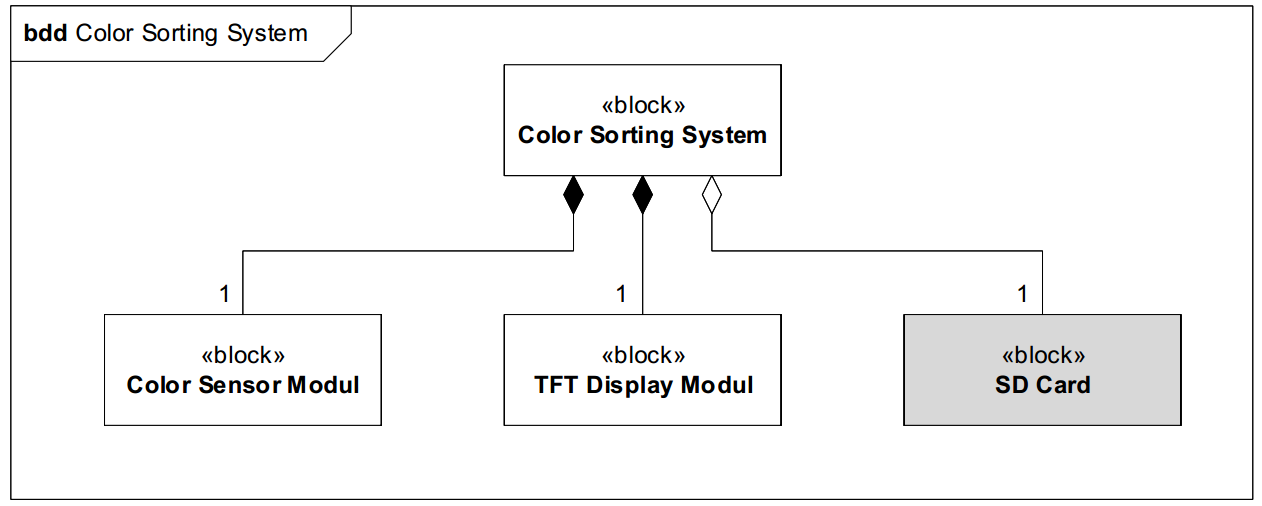
\includegraphics[width = 400pt]{Img/ColorSortingSystem_BDD.png}
	\caption{Color Sorting System BDD}
	\label{fig:ColorSortingSystem_BDD}
\end{figure}

\textbf{TFT Display Module:} \\
Har til opgave at modtage data fra Color Sensor Module og vise brugeren på baggrund af det modtaget data, antallet af hver enkelt farve målt, samt det totale antal farver. Dette modul skulle også havde haft ansvaret for at sende data til SD-kortet, hvis den del var blevet implementeret. 
\\\textbf{Color Sensor Module:} \\
Har til opgave at måle farven placeret under Color Sensoren, samt sende informationen videre til TFT Display Module.
\\\textbf{SD-Kort:}\\
Et SD kort som var tiltænkt at kunne opbevare data som efter systemet slukkes. Dette blev dog taget ud af system. Hvilket visualiseres ved den grå farve i BDD’et.  

\subsection{Blokinteraktion}

På \autoref{fig:ColorSortingSystem_IBD} nedenfor ses det overordnede IBD for systemet. IBD’et viser de forskellige hardwareblokke i systemet og deres interaktion mellem hinanden. Interaktionen mellem blokkene bliver beskrevet mere detaljeret under dokumentationen for de enkelte blokke. I forhold til det overordnede BDD på \autoref{fig:ColorSortingSystem_BDD} har vi valgt at vise hvilke hardware blokke de enkelte moduler består af, for at give et indblik i interaktionen internt i modulerne. 

\begin{figure}[H]
	\centering
	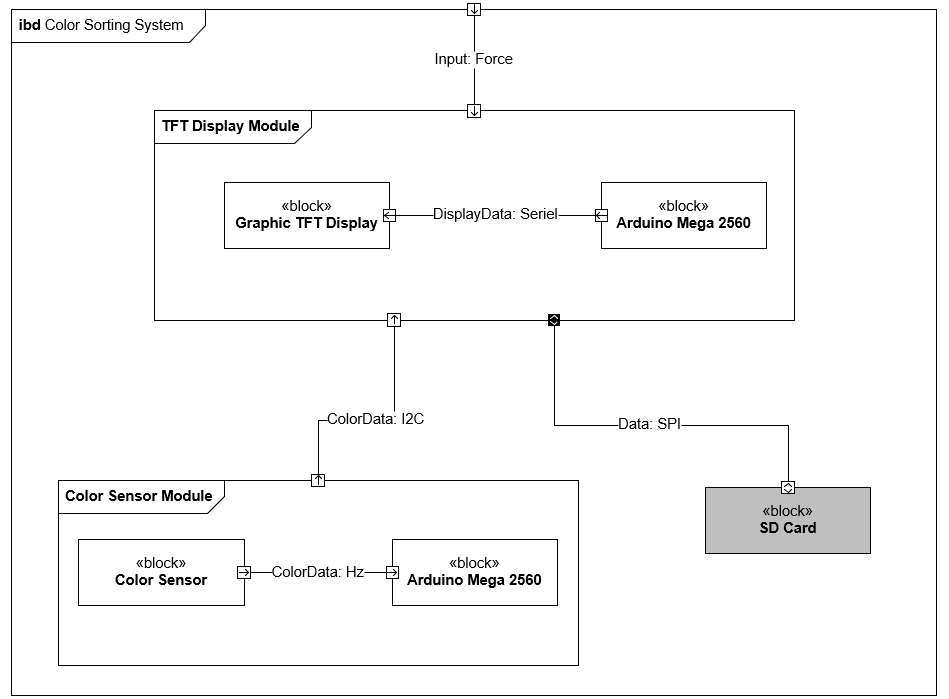
\includegraphics[width = 500pt]{Img/ColorSortingSystem_IBD.png}
	\caption{Color Sorting System IBD}
	\label{fig:ColorSortingSystem_IBD}
\end{figure}
\include{Chapters/Teori/Teori}
%!TEX root = ../../Main.tex
\graphicspath{{Chapters/Struktur/}}
%-------------------------------------------------------------------------------

\section{TFT Display Module}
TFT Display modulets primære opgave er både at fungere som visuel grænseflade til brugeren, samt at fungere som et slags kontrol modul for hele systemet. Kontrol modul forstået på den måde, at når bruger trykker på knappen på boardet vil det trigger et interrupt, som henter data fra Color Sensor Modulet, optæller den hentede information og displayer det for brugeren.\\ Dette modul afsnit vil beskrive TFT Display modulets funktionalitet, samt overvejelser omkring analyse og design både hardware, softwaremæssigt. I dette afsnit vil kommunikationen mellem TFT Display modulet og resten af systemet også blive beskrevet. 

\subsection{Hardware}
I arkitekturfasen gik den første overvejelse på hvilket display vi skulle benytte som grænsefladen til brugeren. Vi ønskede et displayet som kunne vise farver og havde en nogenlunde opløsning for give en god visuel oplevelse for brugeren. Da vi først havde opsat kravene for vores display, var selve valget ikke særligt svært. I undervisningen har vi arbejdet med ”Graphic TFT Display” fra lektion 4, dette display opfyldte vores ønskede krav angående opløsning samt muligheden for at vise farver. Derfor faldt valgt ret hurtigt på dette display, da det også spillede sammen med vores Arduino 2560. For at kunne påmontere ”Graphic TFT Display” på Arduino Mega 2560, har vi benyttet os af ”ITDB02 Arduino MEGA shield 2.0”. Databladet for dette shield kan læses mere om her i bliagene\cite{man:ITDB02}. I dette datablad er det også markeret hvilke porte ITDB02 shieldet der hører til indgange på displayet.

\subsection{Software}
I og med at dette moduls primære opgave er at være visuel grænseflade for brugeren, har langt det meste arbejde med dette modul lagt i softwaren. 
Hvis man kigger på Graphic TFT Display, kan den fungere i fire forskellige MCU-Interface modes, hvilket simpelt betyder, hvor stor en bus-interface man ønsker at arbejde med. Vi har valgt at arbejde med 16-bit bus-interface, hvordan vi sætter dette, bliver også beskrevet i dette afsnit. 

\begin{figure}[H]
	\centering
	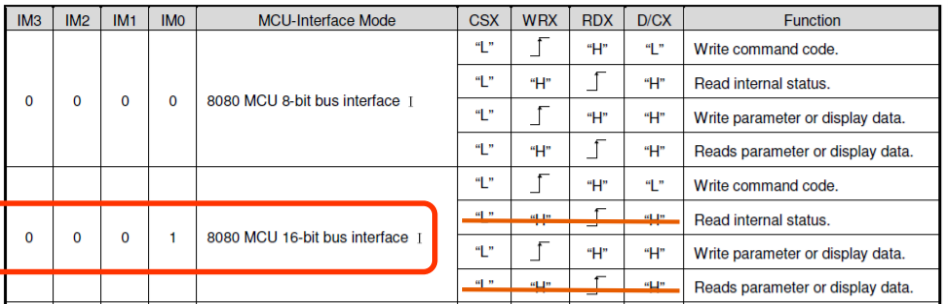
\includegraphics[width = 400pt]{Img/MCU-Interface_Mode.png}
	\caption{MCU-Interface Mode}
	\label{fig:MCU-Interface_Mode}
\end{figure}

I og med at vi udelukkende ønsker at skrive til vores display, vælger vi at ignorere læse kommandoerne, altså retur beskederne som displayet kan give, og udelukkende fokusere på skrive kommandoerne. Derfor er RDX altid sat høj.
Først implementerede vi WriteCommand i vores kode som ses nedenfor.


\begin{lstlisting}
void WriteCommand(unsigned int command)
{
	DATA_PORT_LOW = command;

	DC_PORT &= ~(1<<DC_BIT);
	CS_PORT &= ~(1<<CS_BIT);
	WR_PORT &= ~(1<<WR_BIT);
	
	_NOP();
	WR_PORT |= (1<<WR_BIT);
	_NOP();
}

\end{lstlisting}


Som det ses på figur \autoref{fig:MCU-Interface_Mode} fra databadet\cite{man:ILI9341} side 27, skal DCX og CSX sættes lavt, samt trigger kommandoen på WRX stigende flanke - derfor sættes WRX lav til at starte med. På \autoref{fig:Timedelays} nedenfor ses et skema over de tidsforsinkelser der opstår, ved forskellige operationer. Her ses det at når WRX sættes lav, opstår der en forsinkelse på min 15ns. Derfor er der indsat en NOP() funktion i koden. "NOP" står for ”No Operation”, som vil sige at programmet laver ingenting i en cyklus. Med en MCPU frekvens på 16Mhz svare det til 62,5ns. Herefter sættes WRX høj igen for at trigger kommandoen efterfulgt af endnu en NOP() funktion, da der opstår samme forsinkelse når WRX sættes høj.

\begin{figure}[H]
	\centering
	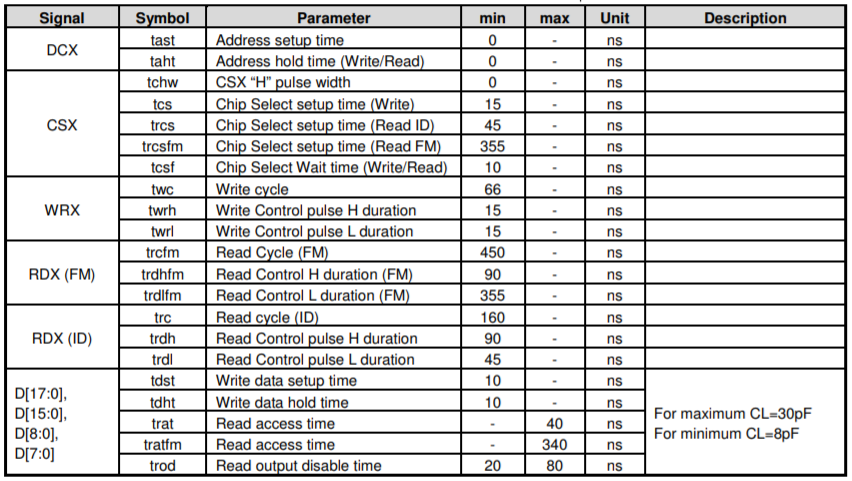
\includegraphics[width = 450pt]{Img/Timedelays.png}
	\caption{Tidsforsinkelser}
	\label{fig:Timedelays}
\end{figure}


Dernæst implementerede vi WriteData, som tilnærmelsesvis ligner WriteCommand bortset fra at DCX skal sættes høj i stedet for lav. Koden for WriteData ses lige nedenfor. Data bliver bitshiftet 8 gang på linje 3, da kun er de 8 LSB der bliver aflæst. På samme måde som WriteCommand trigger WriteData på en stigende flanke på WRX, derfor sættes WRX først lav og dernæst høj, med indsat NOP() funktioner for at tage højde for tidsforsinkelser. 

\begin{lstlisting}
void WriteData(unsigned int data)
{
	DATA_PORT_HIGH = data >> 8;
	DATA_PORT_LOW = data;

	DC_PORT |= (1<<DC_BIT);
	CS_PORT &= ~(1<<CS_BIT);
	WR_PORT &= ~(1<<WR_BIT);

	_NOP();
	WR_PORT |= (1<<WR_BIT);
	_NOP();
}
\end{lstlisting}


I vores DisplayInit() som vi kalder en gang i koden til at Initialisere displayet, koden ses lige nedenfor. Først sættes vores Control Pins som outputs og høje. Port D bit 3 bliver sat lavt, så den er klar til at læse, når brugeren trykker på interrupt-knappen. Dernæst bliver RST sat lav i 300ms, det skyldes at der i databladet\cite{man:ILI9341} på side 230 står minimum 120ms, så det er sat til 300ms for at være på den sikre side. Efter vi igen sætter RST høj, skal vi igen vente 120ms før vi må kalde SleepOut Command. Derfor indsættes et delay på 130ms. Herefter vækkes displayet med Sleepout() kommandoen efterfulgt af Displayon(). Begge disse kommandoer er at finde i databladet\cite{man:ILI9341} på side 83. Den kommando der bliver sendt til MemoryAccessControl() sørger for at sætte rækkefølgen til BGR i stedet for RGB. Til sidst bliver en kommando sendt til InterfacePixelFormat(), denne kommando fortæller displayet at vi ønsker at køre med 16bit pr. pixel se side 134 i databladet\cite{man:ILI9341}. 


\begin{lstlisting}
DisplayInit()
{
	DDRG |= 0b00000111;
	DDRD |= 0b10000000;
	DDRD &= 0b11111011;
	DDRA = 0xFF;
	DDRC = 0xFF;
	PORTG |= 0b00000111;
	PORTD |= 0b10000000;
	PORTD &= 0b11111011;
	
	RST_PORT &= ~(1<<RST_BIT);
	_delay_ms(300);

	RST_PORT |= (1<<RST_BIT);
	_delay_ms(130);
	
	SleepOut();

	DisplayOn();

	MemoryAccessControl(0b00001000);
	
	InterfacePixelFormat(0b00000101);
}
\end{lstlisting}


Efter at have initialiseret og opsat displayet efter eget ønske. Var den næste opgave at kunne skrive tal og bogstaver ud på vores display. Til dette benyttede vi os af et program ved navn ’TheDotFactory’. Vi fik programmet til at udskrive et kæmpe array, som indeholder alle symboler, tal samt bogstaver vi kunne have brug for. Sammen med et tilhørende array, der fortæller længden af hvert symbol samt dens offset. Disse to arrays genereret af programmet ’TheDotFactory’ har vi lagt ind i en h-fil ved navn ”DotFactory.h”.
På den efterfølgende \autoref{TFTDisplayFunktioner} vil funktionerne vi har benyttet blive overordnet blive beskrevet, i vores vedlagte kode vil en mere detaljeret gennemgang af koden kunne ses, i form af kommentar til hver linje kode i den vedlagte kode. 


\begin{table}[]
	\centering
	\caption{Funktioner benyttet til TFT Display}
	\label{TFTDisplayFunktioner}
	\begin{tabular}{|l|l|}
		\hline
		\textbf{Navn}         & \textbf{Beskrivelse}                                                                                                                                                              \\ \hline
		WritePixel() & \begin{tabular}[c]{@{}l@{}}Formålet er at bestemme farven for en pixel. Tager imod 3 parameter.\\ Rød 0-31, grøn 0-63, blå 0-31 smider dem ind i write data.\end{tabular} \\ \hline
		SetColomnAddress() & \begin{tabular}[c]{@{}l@{}}Formålet er at kunne skrive til en hel linje lodret på en gang.\\ Tager imod to parameter start og stop.\end{tabular}                                                                                                                                                                         \\ \hline
		SetPageAddress() & \begin{tabular}[c]{@{}l@{}} Formålet er at kunne skrive til en hel linje vandret på en gang.\\ Tager imod to parameter start og stop. \end{tabular}                                                                                                                                                                        \\ \hline
		FillRectangle() & \begin{tabular}[c]{@{}l@{}} Meningen er at fylde et rektangel med én farve.\\ Tager imod syv parametre: start-x, start-y, bredde, højde,\\ rød, blå og grøn.  \end{tabular}  \\ \hline
		getSymbolParameters() &  \begin{tabular}[c]{@{}l@{}} Den tager tre parametre, start x og start y samt længden på det\\ givne symbol. Formået for denne funktion er at opdele alle de\\ nødvendige informationer for et symbol. Så som længen af symbolet\\ i byte, offset i forhold til arrayet fra TheDotFactory, offset i forhold\\ til displayet. Denne information bliver så videregivet til drawSymbol(). \end{tabular}   \\ \hline
		drawSymbol() &  \begin{tabular}[c]{@{}l@{}}Tager information videregivet fra getSymbolParameters(). Finder det\\ givne symbol i arrayet fra TheDotFactory ved hjælp af de videregivet\\ parametre. Herefter gennemgås symbolet bit for bit, og displayet\\ en sort pixel eller hvid pixel alt efter om det er et ’1’ eller ’0’\\ på den givne plads.  \end{tabular}                                                                                                                                                                                         \\ \hline
		writeString() & \begin{tabular}[c]{@{}l@{}} Tager imod en string. Hvorefter den gennemgår denne string symbol\\ for symbol og kalder getSymbolParameters () som videre kalder\\ drawSymbol() på hvert symbol. Med mindre at symbolet er et\\ mellemrum, så plusses x-positionen med seks.  \end{tabular}                                                                                                                                                                                         \\ \hline
		writeInt() &  \begin{tabular}[c]{@{}l@{}} Tager imod en long int. Hvorefter den int bliver lagt over i et array.\\ Og på hver plads i dette array bliver getSymbolParameters kaldt,\\ efter det første tal er detekteret.   \end{tabular}                                                                                                                                                                                         \\ \hline
		\begin{tabular}[c]{@{}l@{}} DrawRed(),\\ DrawGreen(),\\ DrawBlue() \end{tabular}  &  \begin{tabular}[c]{@{}l@{}} Meningen med denne funktion er at vise en søjle i enten farven rød,\\ grøn eller blå alt efter hvilken af disse tre funktioner der bliver kaldt.\\ Over denne søjle skal så skrives et tal, som følger søjlens højde.\\ Funktionerne modtager to int, den første int angiver tallet som skal\\ stå over søjlen, den anden int angiver højden på søjlen. Tallet\\ bliver vist ved hjælp af funktionen writeInt(), og søjlen bliver vist ved\\ hjælp af funktionen FillRectangle(). Den eneste forskel på disse tre\\ funktioner er farven af søjlen.  \end{tabular} \\ \hline
		drawTotal() &  \begin{tabular}[c]{@{}l@{}} Meningen med denne funktion er at den skal tage tre parametre som\\ antallet af hver farve detekteret. Disse tre parametre bliver så lagt\\ sammen i en totalCount variable, og udregnet hvor stor en procentdel\\ de hver udgør at det samlet antal optællinger. Den procentdel\\ udgør så hvor høj hver enkel søjle skal være. Så vil DrawRed(),\\ DrawGreen() og DrawBlue() blive kaldt hvor de tre parametre vil\\ være tallene over søjlerne, højden vil være den udregnede\\ procentdel og totalCount vil blive vist i øverste højre hjørne\\ ved hjælp af writeInt().  \end{tabular}                                                                                                                                                                                         \\ \hline
	\end{tabular}
\end{table}
\newpage



På \autoref{fig:Flowchart_TFTDisplay_SW} ses et lille flow chart over main koden til TFT Display Modul. Modulet bliver trigget af at brugeren trykker på knappen. Det får modulet til at hente sit input igennem en I2C forbindelse fra Color Sensor Module, som vil blive mere uddybet i det efterfølgende afsnit. Det input bliver så undersøgt, og alt efter hvilket char 'R', 'G' eller 'B' der bliver modtaget optælles den tilhørende conut til den farve, hvorefter displayet bliver clearet og det nye resultat bliver vist. Så er modulet klar til et nyt input.
\begin{figure}[H]
	\centering
	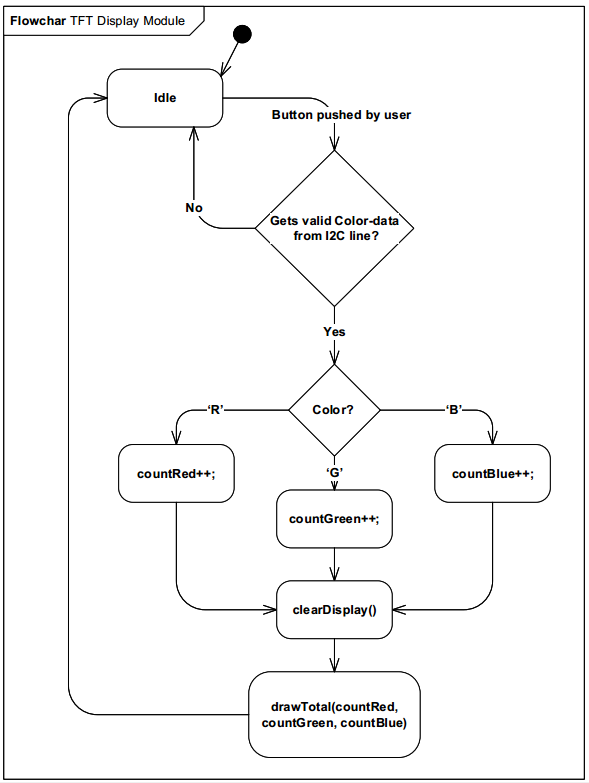
\includegraphics[width = 300pt]{Img/Flowchart_TFTDisplay_SW.png}
	\caption{Flowchart TFT Display software}
	\label{fig:Flowchart_TFTDisplay_SW}
\end{figure}


\subsection{Test}
Efter modulet stod færdig blev en enhedstest af modulet lavet resultatet af dette ses på \autoref{fig:TFT_Display_Module_test}. I testen blev countBlue og countGreen hver plusset op 1 og countRed blev pludset op med 2 en gang i sekundet. Som det kan ses passer vores procentvise fordeling af søjlerne. Blå og grøn søjle har samme højde og den røde søjle er dobbelt så høj. Det er kun i enhedstesten af vi plusser count variablerne op en gang i sekundet. I det færdige system vil denne data komme fra I2C linjen. 


\begin{figure}[H]
	\centering
	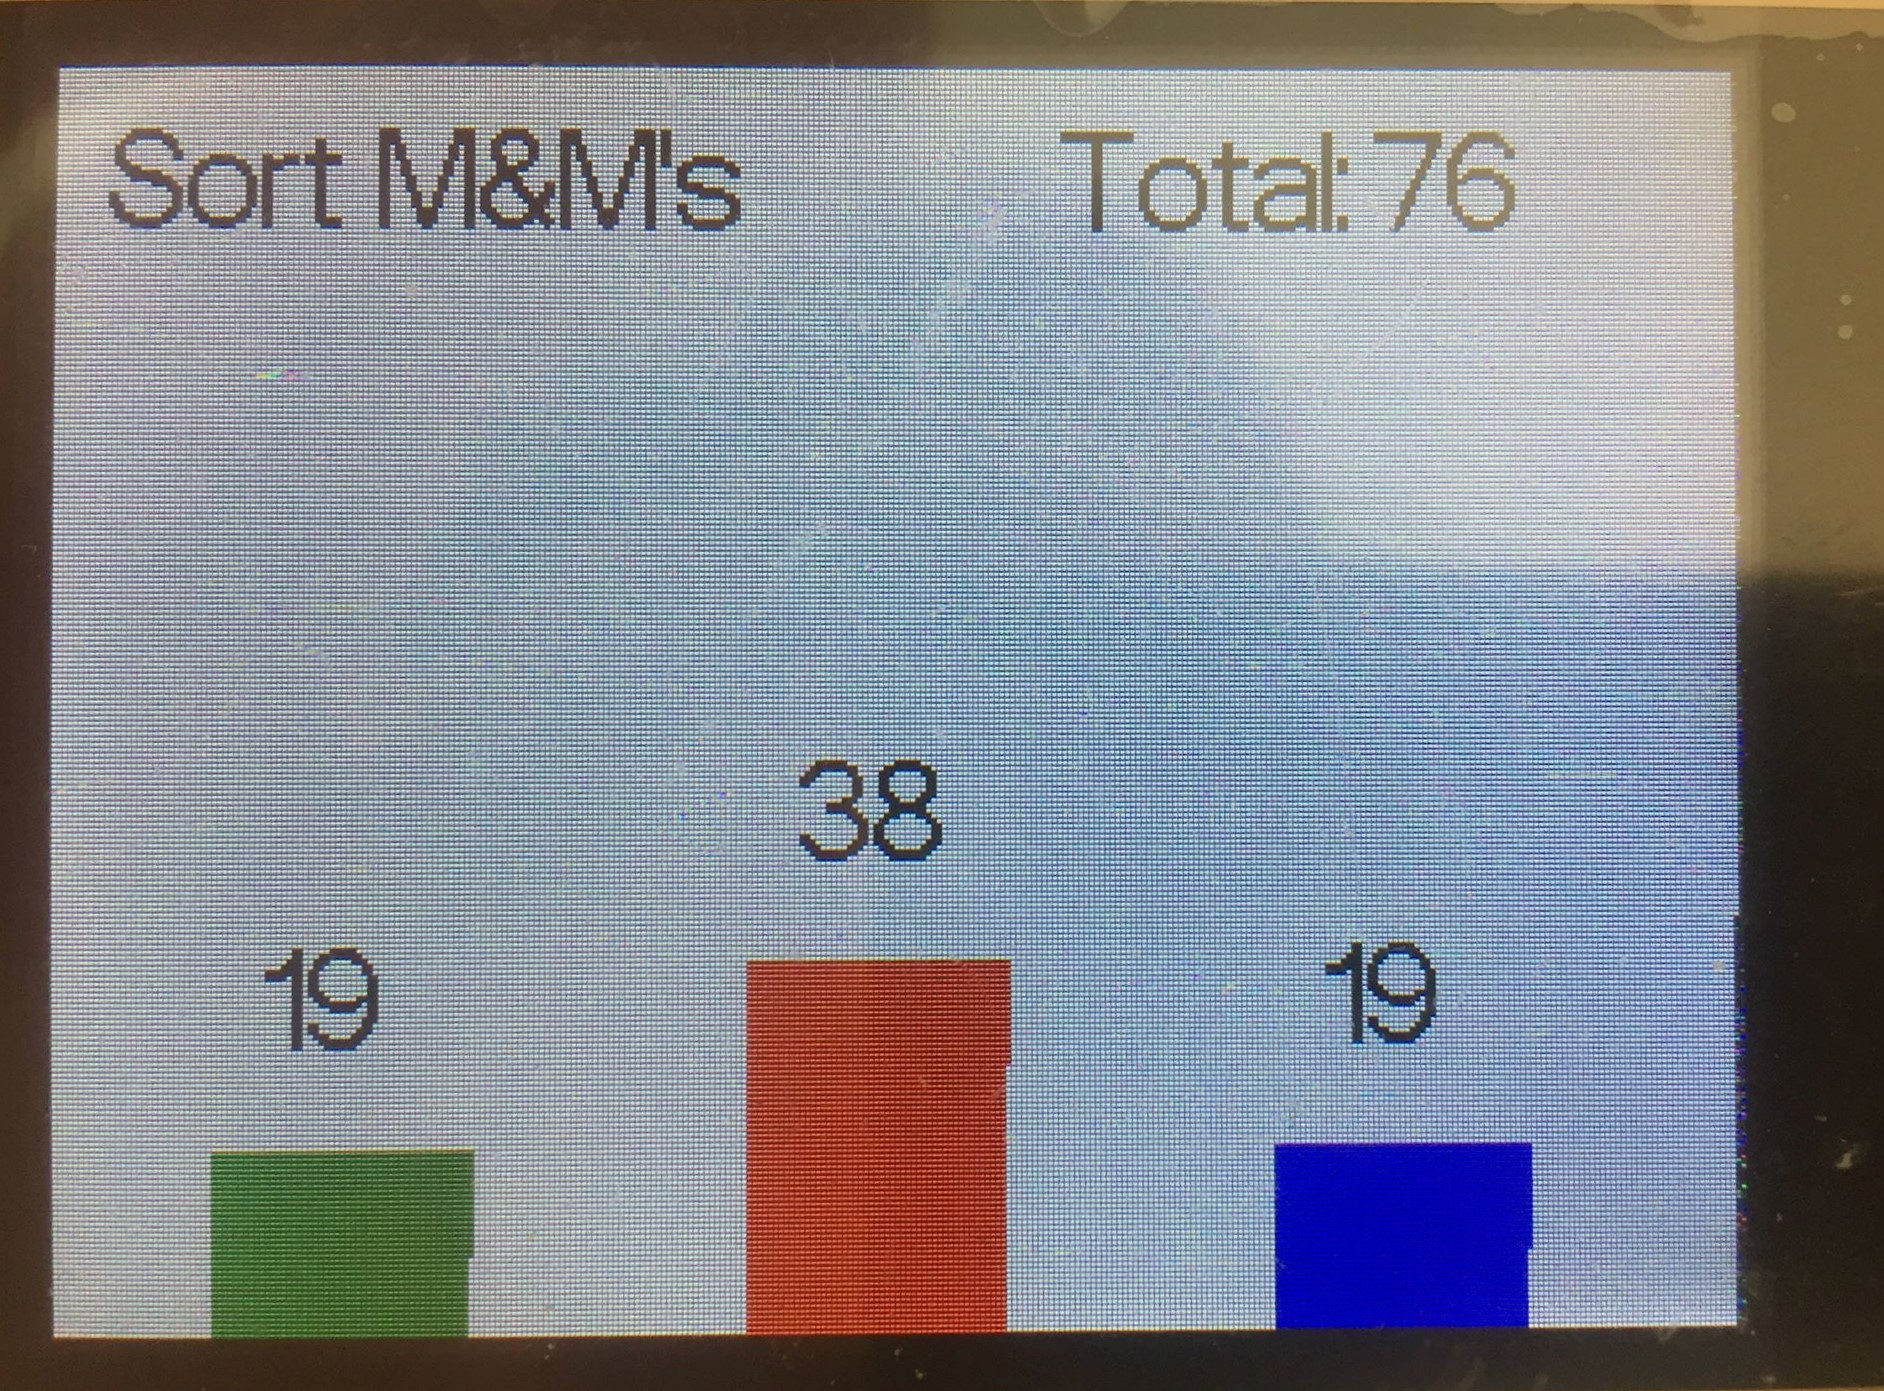
\includegraphics[width = 300pt]{Img/TFT_Display_Module_test.jpg}
	\caption{TFT Display Module enhedstest}
	\label{fig:TFT_Display_Module_test}
\end{figure}

%!TEX root = ../../Main.tex
\graphicspath{{Chapters/Matlab/}}
%-------------------------------------------------------------------------------







%!TEX root = ../../Main.tex
\graphicspath{{Chapters/Test/}}
%-------------------------------------------------------------------------------


\section{I2C kommunikation}
Til at starte med havde gruppen ikke planer om at inkorporere I2C i CSS, da den bedste og mest simple løsning var at have både TFT skærmen og Color Sensoren sat til samme Arduino. Dette viste sig ikke at kunne lade sig gøre, da skærmen og sensoren begge bruger pin 49, hvilket gjorde at systemet ikke fungerede. Desværre kunne vi ikke bruge andre pins til sensoren, da de to input capture pins der er at vælge imellem, begge sad i vejen for skærmen. Derfor valgte gruppen at splitte systemet op og anvende I2C. På grund af denne ekstra arbejsbyrde, blev SD kort implementationen nedprioriteret.

\subsection{I2C master}
Masteren blev valgt implementeret på TFT display modulet, da det ikke ville give mening at lade sensor modulet sende kommandoer til display modulet. Istedet for sendes der en char fra slaven, som repræsenterer en farve. Inspiration til at implementere I2C i systemet, blev fundet fra det udleverede undervisningsmateriale fra timen samt denne video\cite{mic:I2CVideo}.

Før masteren kan bruges skal den først initiereres. Dette sker ved at sætte bestemte dataregistre op rigtigt. Først bestemmer man hvilken clock SCL skal have. SCL kan udregens på følgende måde:

\begin{equation}
SCL= \frac{CPU}{16+2(TWBR)*4^{TWPS}} 
\end{equation}

Gruppen har valgt at en clock på 500KHz.Kravene til clokcen er at den er 16 gange lavere end slavens cpu clock, ifølge megea 2560 datablad og at den kan nå at vores farve data hurtigt nok. Da slaven kører med 16MHz, opfylder den første krav, og da hastigheden er langt over hvad der er nødvendigt for at kunne sende enkelte chars, endte valget på 500KHz. 

\begin{figure}[H]
	\centering
	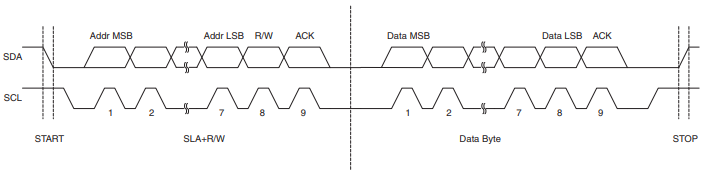
\includegraphics[width = 450pt]{Img/I2CTiming.png}
	\caption{I2C timing diagram}
	\label{fig:I2CTIming}
\end{figure}

Til udviklingen af masteren har et timing diagram over I2C protokollen, se \autoref{fig:I2CTIming}, været utrolig nyttig. Ved hjælp af dette diagram har gruppen kunne sende korrekte beskeder over I2C. 

For at have en så overskuelig kode som overhovedet muligt, er der blevet lavet funktioner der kan generere ACK, NACK, WAIT, START og STOP. Disse funktioner er så brugt i vores i2c\_master\_receive() funktion. Et Kodeudsnit af denne funktion kan findes nedenunder:

\newpage

\begin{lstlisting}
i2c_master_start();
while(transfer && i < 250)
{
	
	switch (i2c_master_status())
	{
		//SLA+R will be transmitted
		//ACK or NOT ACK will be received
		case 0x08:
		TWDR = address_r;
		i2c_master_ack();
		i2c_master_wait();
		break;
		
		// Data byte will be received and NOT ACK will be returned
		// Data byte will be received and ACK will be returned
		case 0x40:
		i2c_master_nack();
		i2c_master_wait();
		break;
		
		// Data byte will be received and NOT ACK will be returned
		// Data byte will be received and ACK will be returned
		case 0x50:
		data = TWDR;
		transfer = 0;
		break;
		
		// Repeated START will be transmitted
		// STOP condition will be transmitted and TWSTO Flag will be reset
		// STOP condition followed by a START condition will be transmitted and TWSTO Flag will be reset
		case 0x58:
		data = TWDR;
		transfer = 0;
		break;
	}
	i++;
}
i2c_master_stop();
\end{lstlisting}

Som det ses i koden bliver i2c\_master\_status() hele tiden tjekket på, for at finde ud af om slaven reagerer på nogle af kommandoerne fra masteren. Status funktion tjekker TWSR registeret og AND'er det med 0xF8, for at sætte de tre sidste bits til 0. I mega 2560 datablad kan der findes en tabel over hvad de forskellige status koder står for\cite{man:mega2560Kap24}. I kode udsnittet står de som kommentarer over hver case.

\subsection{I2C slave}
Ligesom masteren skal slave også initialiseres, ved at sætte nogle bestemte dataregistre op. TWAR registeret bestemmer slavens adresse, i vores tilfælde er den sat til 40. TWCR registeret bestemmer hvilken slave mode den skal sættes i, i vores tilfælde er det slave transmitter mode. Det vil sige at slaven kun skal kunne sende data til masteren, og ikke modtage data. 

Når slaven er sat op i transmitter mode, bliver der gjort brug af et interrupt, der trigger når i2c interfacet bliver brugt. Når et interrupt bliver triggered, køres vores interrupt rutine, som kan ses nedenunder:

\begin{lstlisting}
if(i2c_slave_addressed())
{

switch(i2c_slave_status())
{
// Own SLA+R has been received;
//ACK has been returned
case 0x60:
i2c_slave_ack();
break;

//Arbitration lost in SLA+R/W as
//Master; own SLA+R has been received;
//ACK has been returned
case 0x80:
data = TWDR;
i2c_slave_ack();
transfer = 0;
break;

// Data byte in TWDR has been
//transmitted; ACK has been received
case 0xA8:
TWDR = dataToSend; //data send to master
i2c_slave_ack();
break;

// Last data byte in TWDR has been
//transmitted (TWEA = 0)
// ACK has been received
case 0xC0:
transfer = 0;
i2c_slave_ack();
break;
}
}\end{lstlisting}

Interrupt rutinen minder meget om masterens receive funktion. Den tjekker hele tiden på status registeret(TWSR), for at holde styr på hvor langt den er i I2C processen. dataToSend indeholder en char med information om hvilken farve color sensoren har opfanget. 

\subsection{Test}
Til test af I2C, har vi gjort brug af en logic analyzer, som bruges til at afkode beskeder der sende med forskellige protokoller. Det har været en stor hjælp til at finde fejl i vores software. Blandt andet fandt vi ud af at hvis UART og I2C blev brugt samtidig, skabte det en stor nok forsinkelse i I2C protokollen. Dette skyldes at der ikke blev sendt et ACK på det rigtige tidspunkt. 

\begin{figure}[H]
	\centering
	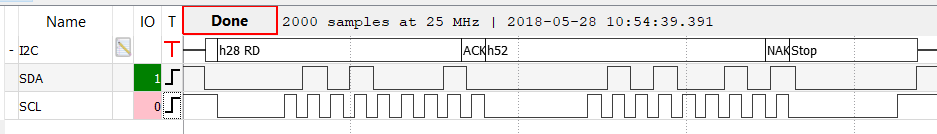
\includegraphics[width = 450pt]{Img/I2C_logic.png}
	\caption{Logic analyzer for I2C}
	\label{fig:I2C_Logic}
\end{figure}

På figuren ovenfor kan man se en perfekt I2C transmission. På figuren kan man se at et start condition, starter transmissionen, hvorefter adressen på slaven bliver sendt og at R/Wbit bliver sat højt, hvilket betyder READ. Derfter kommer dataen. I dette tilfælde bliver der sendt h52, hvilket i ASCII svarer til bogstavet 'R'. Et NACK kommer bagefter for at signallere at der ikke er mere data, hvorefter et stop condition blever genereret. Testopstillingen kan ses nedenunder.

\begin{figure}[H]
	\centering
	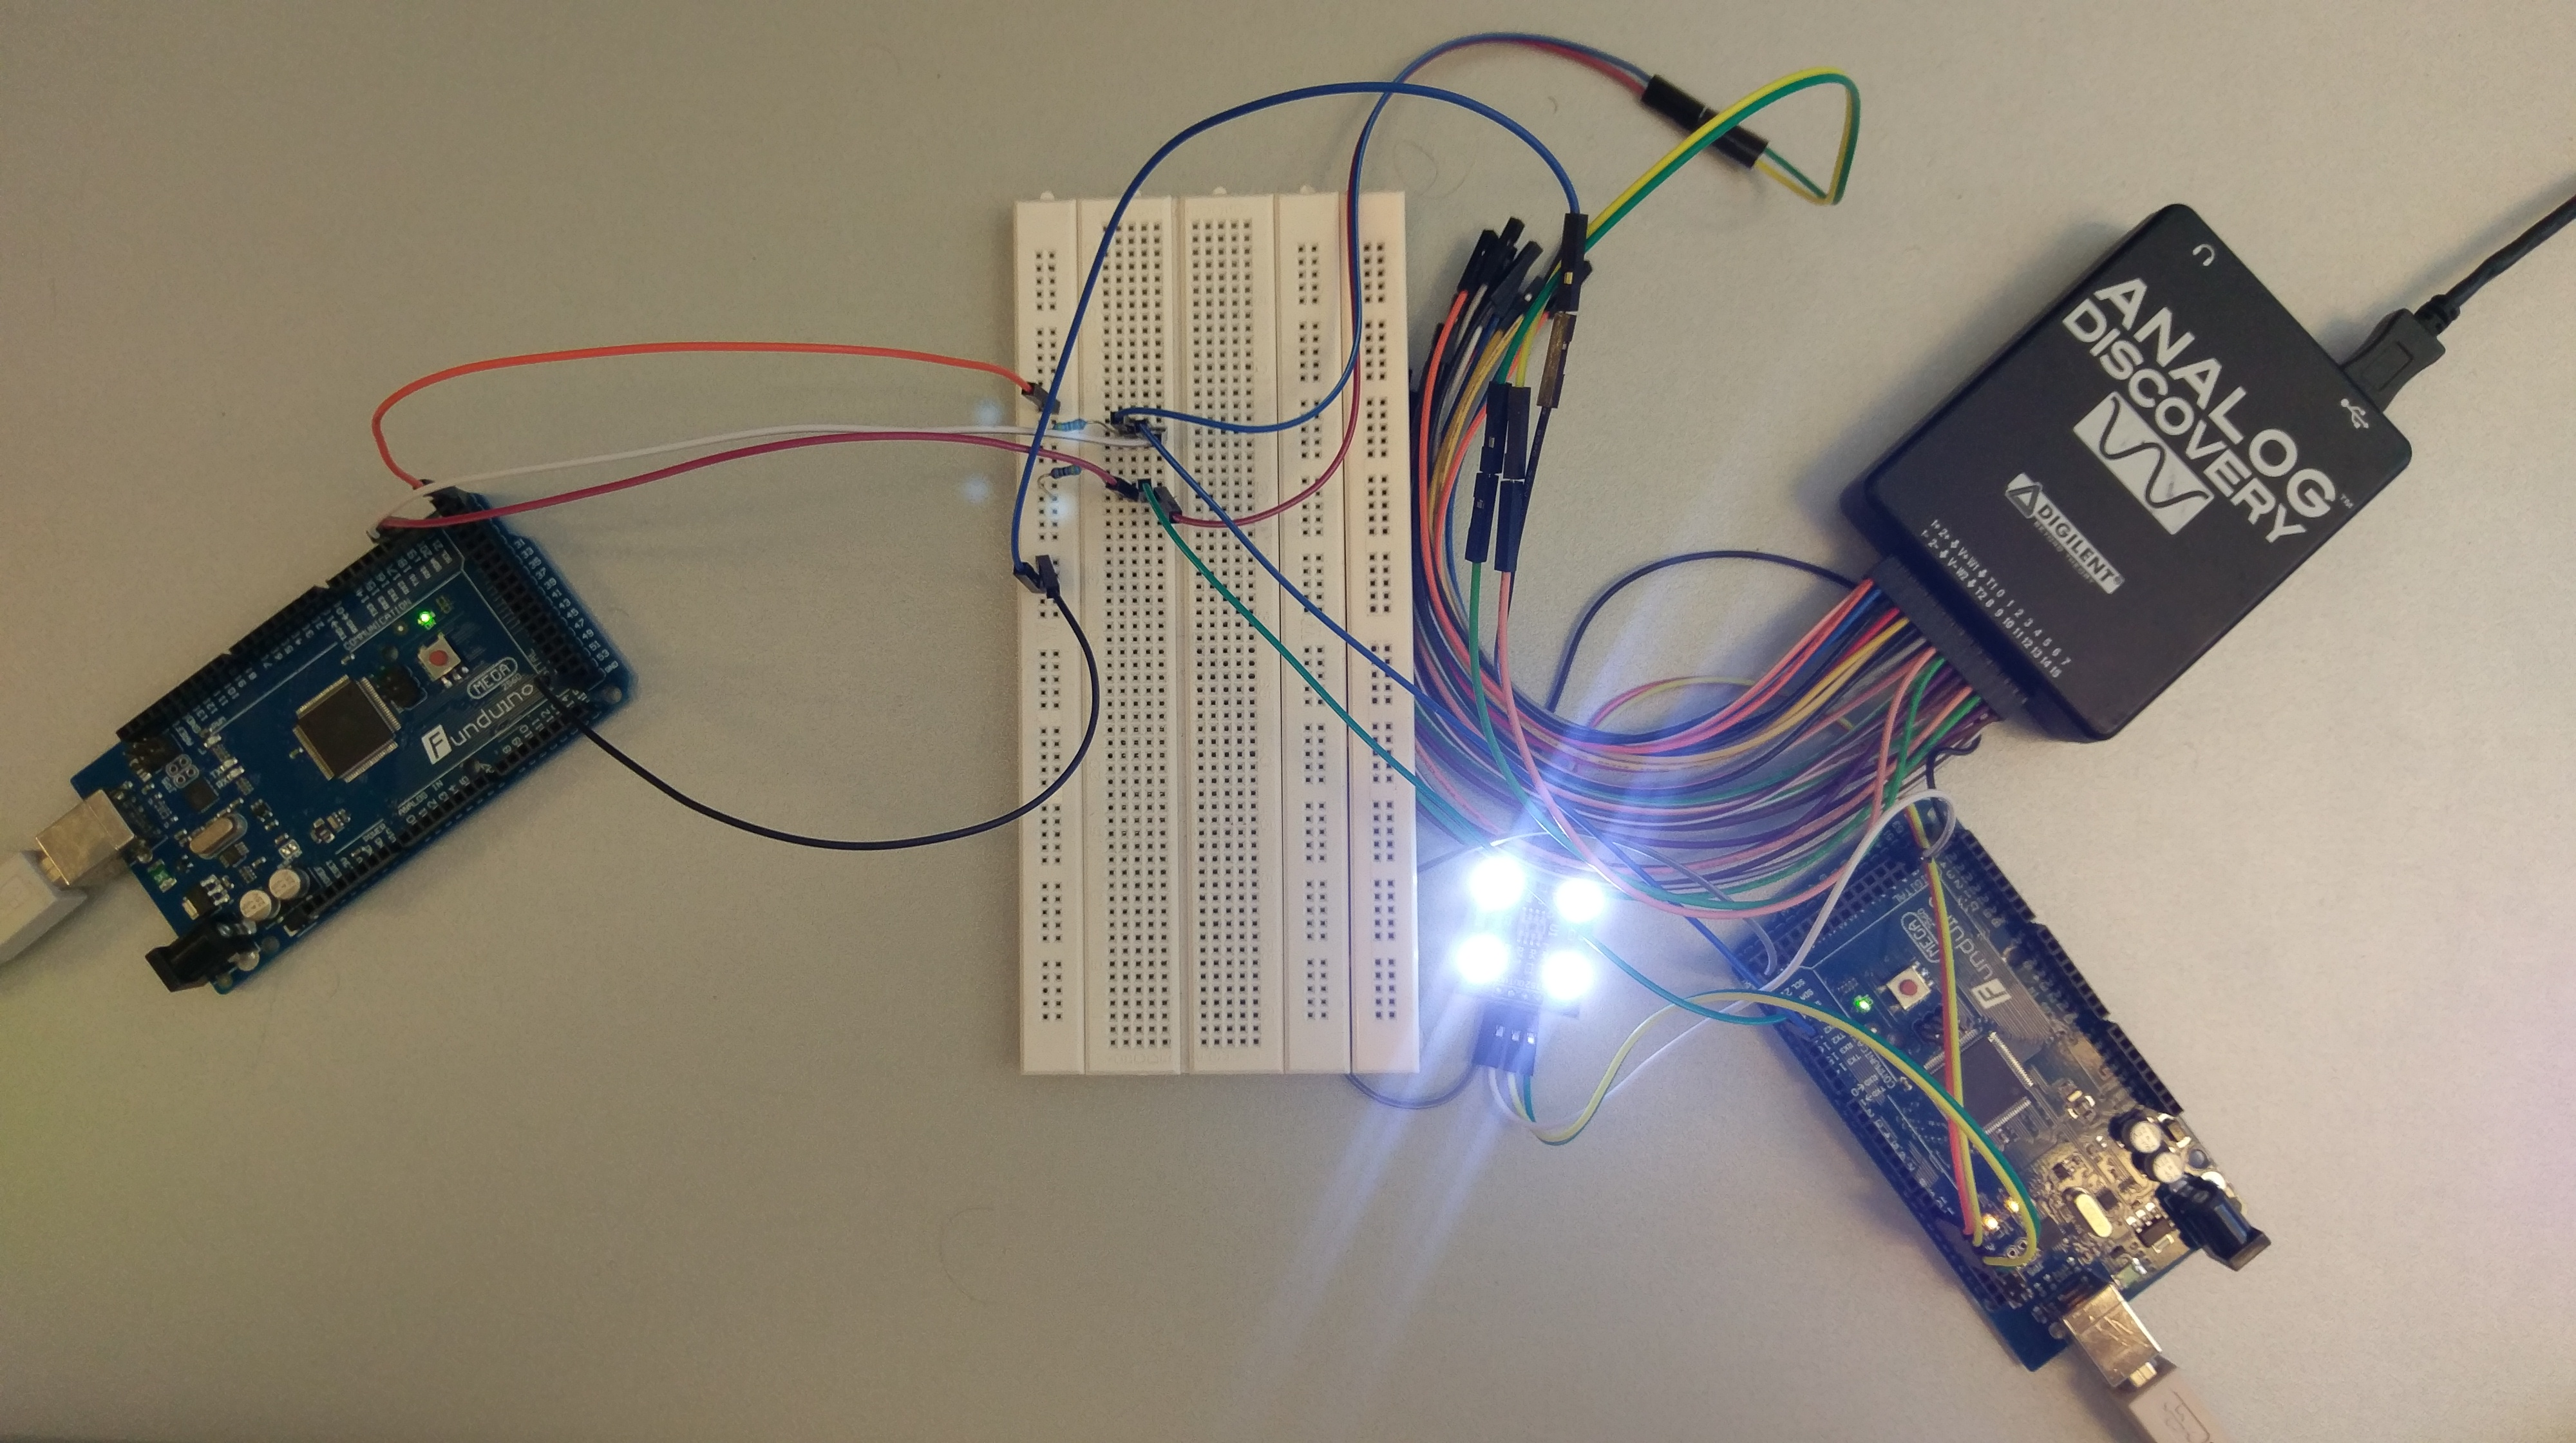
\includegraphics[width = 450pt]{Img/TestOpstilling.jpg}
	\caption{Test opstilling af I2C}
	\label{fig:I2C_Test}
\end{figure}



%!TEX root = ../../Main.tex
\graphicspath{{Chapters/Alternative_Loesninger/}}
%-------------------------------------------------------------------------------


\section{Alternative Løsninger}
I dette afsnit vil fordele og ulemper for forskellige alternative løsninger blive diskuteret.

\subsection{Valg af Kommunikation}
Istedet for I2C som kommunikationsprotokol var SPI oplagt. SPI har den fordel at være hurtigere, men kræver 4 ledninger. SPI er hurtigere fordi protokollen kan køre full-duplex, hvorimod I2C er half-duplex. Men da antallet af ledninger var mindre og at vores behov for overførelseshastighed var opfyldt med I2C, valgte vi denne protokol.

Det skal siges at det aldrig var meningen at indbringe to arduinoer, da det ville gøre system mere kompleks uden at give ekstra værdi, men da sensor og skærm ikke kunne komme til at fungere op samme arduino, endte valget på I2C som en løsning på det problem.

\subsection{Valg af color sensor}
Da projektet ikke vil kunne realiseres uden en color sensor, og at der ikke var andre end LC technology TC3200 sensoren på lager, var den det oplagte valg. Men efter at have arbejdet med den og testet den, fandt vi hurtigt ud af at den ikke var specielt præcis i sin målinger. Derfor vil en sensor af bedre kvalitet have være at foretrække, men som proof of concept fungerer den nuværende sensor fint. 

\subsection{Valg af skærm}
Istedet for en farve-skærm, kunne vi have valgt et alphanumerisk display, men dette vil være en betydelig nedgradering fra den nuværende farve-skærm. Derudover vil det ikke være muligt at vise søjlediagrammer på et alphanumerisk display. Desuden er der indbygget touch i farve-skærmen, som i fremtiden vil kunne inkorporeres, hvis dette ønskes.

\include{Chapters/CSS_test/Css_test}
%!TEX root = ../../Main.tex
\graphicspath{{Chapters/Konklussion/}}
%-------------------------------------------------------------------------------

\section{Diskussion}
Igennem projektet har vi stødt på flere forskellige problemer. Et af de meget tidskrævende problemer var identifikation af overføringsfunktionen for vores bil. Vores bil accelerede op til max hastighed utrolig hurtigt, hvilket resulteret i at det transiente område af \autopageref{fig:Motor_deg_graf} blev meget smalt. Det betød at vi kun havde nogle få samples til at bestemme overfæringsfunktionen ud fra. Desuden var der også problemer den første motor, som havde en masse slør der resulterede i at den "hoppede", hvilket teknisk set betød at vi havde en ekstra pol. Vi valgte dog at prøve en anden motor, som viste sig næsten at løse problemt. 
EV3 hardwaren har også voldt os problemer. Det har især været at få forbindelse til EV3 over wifi. Det viste sig at være et problem på en af telefonerne, så det blev løst ved at skifte telefon.
Grundet de mange problemer har vi ikke nået så langt som vi havde forventet, dog er der blevet udarbejdet et godt fungerende kontrolsystem.

\section{Konklussion}

Vi har i dette projekt, fået stillet nogle overordnede krav, til hvad vores regulerings system skulle indeholde. Vi har fra staten ville gribe dette projekt simpelt an, da vi hellere ville stå i en situation, hvor projektet skulle udvides, frem for indskrænkes. Efter forskellige test af sensorer og aktuatorer, endte vores system med at bestå af en motor og en encoder, som skulle være i stand til at køre en specifik afstand, upåvirket af vægt eller andre forstyrrelser.\\
Igennem arbejdet med dette system, kom vi bl.a. omkring identifikation af det faktiske system, placering af poler for at opnå ønsket overshoot og settling time, samt design af observer både i kontinuere og diskret domæne. \\
Selvom vi i gruppen løb ind i en del problemer, bl.a. at oprette forbindelse til HW og fjerne steady state fejlen i det diskrete domæne, fik vi alligevel implementeret en velfungerende observer i det diskrete domæne på vores Lego bil, som fungerede efter hensigten. Grundet tidsmangel og mange problemer undervejs, nåede gruppen aldrig at implementere adaptiv regulering af nogen form på systemet. \\
Alt i alt er gruppen meget tilfreds med projektforløbet, da det har været utrolig lærerigt. Det har givet en helt anden indsigt i arbejdet med regulering, end opgaver i timen her givet. 






\begin{flushleft}
	
\end{flushleft}


\bibliographystyle{plain}
\bibliography{Bibliography}	

 
\end{document}